
\section{Evaluation} \label{sec:eval}
In this section, we evaluate our FDEs as a method for MV retrieval. First, we evaluate the FDEs themselves (offline) as a proxy for Chamfer similarity (§\ref{sec:fde-experimental}). In (§\ref{sec:online}), we discuss the implementation of $\name$, as well as several optimizations made in the search. Then we evaluate the latency of $\name$ compared to PLAID, and study the effects of the aforementioned optimizations.



\textbf{Datasets.} Our evaluation includes results from six of the well-studied BEIR \cite{thakur2021beir} information retrieval datasets: MS MARCO \cite{nguyen2016ms} (CC BY-SA 4.0), HotpotQA (CC BY-SA 4.0) \cite{yang2018hotpotqa}, NQ (Apache-2.0) \cite{kwiatkowski2019natural}, Quora (Apache-2.0) \cite{thakur2021beir}, SciDocs (CC BY 4.0) \cite{cohan2020specter}, and ArguAna (Apache-2.0) \cite{wachsmuth2018retrieval}. These datasets were selected for varying corpus size (8K-8.8M) and average number of document tokens (18-165); see (§\ref{app:datasets}) for further dataset statistics. Following \cite{santhanam2022plaid}, we use the development set for our experiments on MS MARCO, and use the test set on the other datasets.  


\textbf{MV Model, MV Embedding Sizes, and FDE Dimensionality.}
We compute our FDEs on the MV embeddings produced by the ColBERTv2 model \cite{santhanam2021colbertv2} (MIT License), which have a dimension of $d= 128$ and a fixed number $|Q|=32$ of embeddings per query. The number of document embeddings is variable, ranging from an average of $18.3$ on Quora to $~165$ on Scidocs. This results in ~2,300-21,000 floats per document on average (e.g. 10,087 for MS MARCO). Thus, when constructing our FDEs we consider a comparable range of dimensions $\dfde$ between ~1,000-20,000. Furthermore,  using product quantization, we show in (§\ref{sec:online}) that the FDEs can be significantly compressed by $32\times$ with minimal quality loss, further increasing the practicality of FDEs.  


\subsection{Offline Evaluation of FDE Quality}
\label{sec:fde-experimental}
We evaluate the quality of our FDEs as a proxy for the Chamfer similarity, without any re-ranking and using exact (offline) search. We first demonstrate that FDE recall quality improves dependably as the dimension $\dfde$ increases, making our method relatively easy to tune. We then show that FDEs are a more effective method of retrieval than the SV heuristic. Specifically, the FDE method achieves Recall$@N$ exceeding the Recall$@$2-4N of the SV heuristic, while in principle scanning a similar number of floats in the search. This suggests that the success of the SV heuristic is largely due to the significant effort put towards optimizing it (as supported by \cite{macavaney2024reproducibility}), and similar effort for FDEs may result in even bigger efficiency gains. Additional plots can be found in (§\ref{sec:additional-plots}). All recall curves use a single FDE instantiation, since in (§\ref{app:variance}) we show the variance of FDE recall is negligible. 



\textbf{FDE Quality vs. Dimensionality.}
We study how the retrieval quality of FDE's improves as a function of the dimension $\dfde$. We perform a grid search over FDE parameters $\reps \in \{1,5,10,15,20\}, \ksim \in \{2,3,4,5,6\}, \dproj \in \{8,16,32,64\}$, and compute recall on MS MARCO (Figure \ref{fig:grid_search}). We find that Pareto optimal parameters are generally achieved by larger $\reps$, with $\ksim,\dproj$ playing a lesser role in improving quality. Specifically, $(\reps,\ksim,\dproj) \in\{ (20,3,8),(20,4,8)(20,5,8),(20,5,16) \}$ were all Pareto optimal for their respective dimensions (namely $\reps \cdot 2^{\ksim} \cdot \dproj$).
While there are small variations depending on the parameter choice, the FDE quality is tightly linked to dimensionality; increase in dimensionality will generally result in quality gains. 
We also evaluate using $k$-means as a method of partitioning instead of SimHash. Specifically, we cluster the document embeddings with $k$-means and set $\varphi(x)$ to be the index of the nearest centroid to $x$. We perform a grid search over the same parameters (but with $k \in \{4,8,16,32,64\}$ to match $B = 2^{\ksim}$). We find that $k$-means partitioning offers no quality gains on the Pareto Frontier over SimHash, and is often worse.  Moreover, FDE construction with $k$-means is no longer data oblivious. 
Thus, SimHash is chosen as the preferred method for partitioning for the remainder of our experiments. 



\begin{figure}[t]
    \centering
 %   \vspace{-2em}
  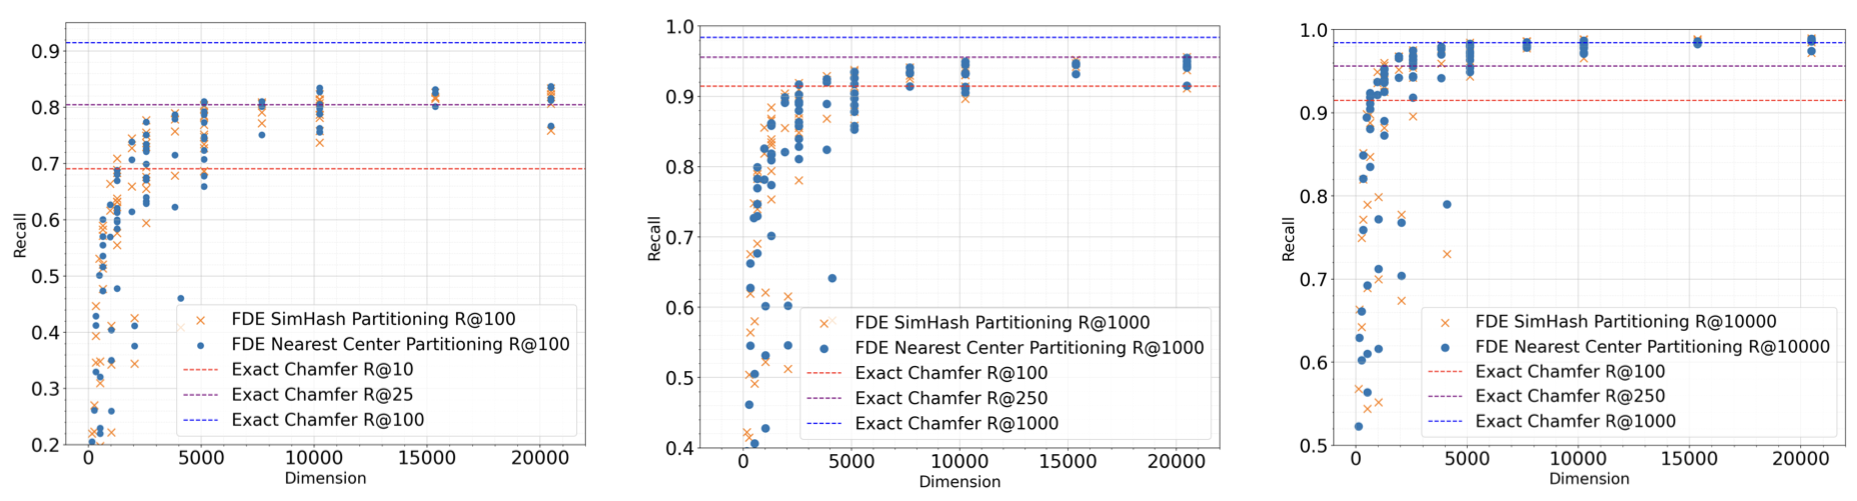
\includegraphics[width=\linewidth]{plots/Grid_Search_Three.png}
    \caption{\small FDE recall vs dimension for varying FDE parameters on MS MARCO. Plots show FDE Recall$@$100,1k,10k left to right.  Recalls$@N$ for exact Chamfer scoring is shown by dotted lines. }
         \label{fig:grid_search} % Add a label (optional)
\end{figure}


\begin{figure}[t]
    \centering
   % \vspace{-1em}
  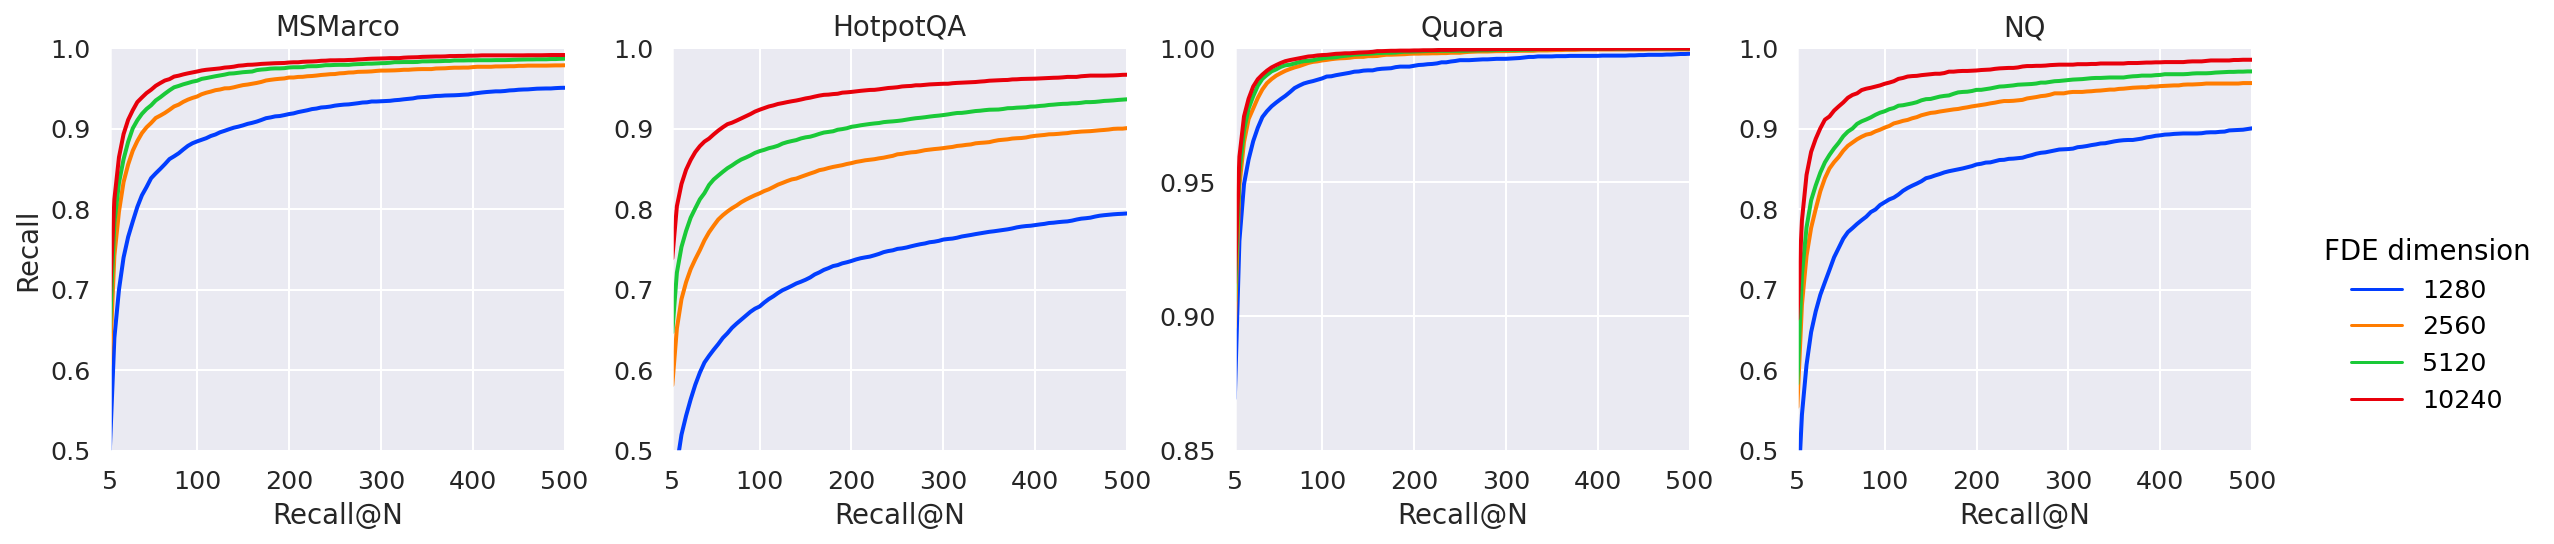
\includegraphics[width=\linewidth]{plots/recall_vs_chamfer.png}
    \caption{\small Comparison of FDE recall versus brute-force search over Chamfer similarity.}
         \label{fig:chamfer} % Add a label (optional)
\end{figure}



In Figure \ref{fig:chamfer}, we evaluate the FDE retrieval quality with respect to the Chamfer similarity (instead of labelled ground truth data).  We compute $1$Recall@$N$, which is the fraction of queries for which the Chamfer $1$-nearest neighbor is among the top-$N$ most similar in FDE dot product. We choose FDE parameters which are Pareto optimal for the dimension from the above grid search. We find that FDE's with fewer dimensions that the original MV representations achieve significantly good recall across multiple BEIR retrieval datasets. For instance, on MS MARCO (where $d\cdot m_{avg} \approx 10K$) we achieve $95\%$ recall while retrieving only $75$ candidates using $\dfde = 5120$.


\paragraph{Single Vector Heuristic vs. FDE retrieval.}
We compare the quality of FDEs as a proxy for retrieval against the previously described SV heuristic, which is the method underpinning PLAID.
Recall that in this method, for each of the $i=1,\dots,32$ query vectors $q_i$ we compute the $k$ nearest neighbors $p_{1,i},\dots,p_{k,i}$ from the set $\cup_{i} P_i$ of all documents token embeddings. To compute Recall$@N$, 
%we collect the relevant document ID's $\ell_{1,i},\dots,\ell_{k,i}$, 
we create an ordered list $\ell_{1,1},\dots,\ell_{1,32}, \ell_{2,1},\dots$, where $\ell_{i,j}$ is the document ID containing $p_{i,j}$, consisting of the $1$-nearest neighbors of the queries, then the $2$-nearest neighbors, and so on. When re-ranking, one firsts removes duplicate document IDs from this list. Since duplicates cannot be detected while performing the initial $32$ SV MIPS queries, the SV heuristic needs to over-retrieve to reach a desired number of unique candidates. Thus, we note that the true recall curve of implementations of the SV heuristic (e.g. PLAID) is somewhere between the case of no deduplication and full deduplication; we compare to both in Figure \ref{fig:sv_mv}. 

 

To compare the cost of the SV heuristic to running MIPS over the FDEs, we consider the total number of floats scanned by both using a brute force search. 
The FDE method must scan $n\cdot \dfde$ floats to compute the $k$-nearest neighbors. For the SV heuristic, one runs $32$ brute force scans over $n\cdot m_{avg}$ vectors in $128$ dimensions, where $m_{avg}$ is the average number  embeddings per document (see §\ref{app:datasets} for values of $m_{avg}$). For MS MARCO, where $m_{avg} = 78.8$, the SV heuristic searches through $32 \cdot 128 \cdot 78.8 \cdot n$ floats. This allows for an FDE dimension of $\dfde =$ 322,764 to have comparable cost! We can extend this comparison to fast approximate search -- suppose that approximate MIPS over $n$ vectors can be accomplished in sublinear $n^\eps$ time, for some $\eps \in (0,1)$. Then even in the unrealistic case of $\eps=0$, we can still afford an FDE dimension of $\dfde = 32\cdot 128 = 4096$.

The results can be found in Figure \ref{fig:sv_mv}. We build FDEs once for each dimension, using $\reps = 40, \ksim = 6, \dproj = d = 128$, and then applying a final projection to reduce to the target dimension (see \ref{app:finalproj} for experiments on the impact of final projections).
On MS MARCO, even the $4096$-dimensional FDEs match the recall of the (deduplicated) SV heuristic while retrieving 1.75-3.75$\times$ \emph{fewer} candidates  (our Recall$@N$ matches the Recall$@$1.75-3.75$N$ of the SV heuristic), and 10.5-15$\times$ fewer than to the non-deduplicated SV heuristic. For our $10240$-dimension FDEs, these numbers are 2.6-5$\times$ and 20-22.5$\times$ fewer, respectively. For instance, we achieve $80\%$ recall with $60$ candidates when $\dfde = 10240$ and $80$ candidates when $\dfde = 4096$, but the SV heuristic requires $300$ and $1200$ candidates (for dedup and non-dedup respectively). See Table \ref{table:sv_mv_table} for further comparisons.



\begin{figure}[t]
    \centering
   % \vspace{-1.5em}
  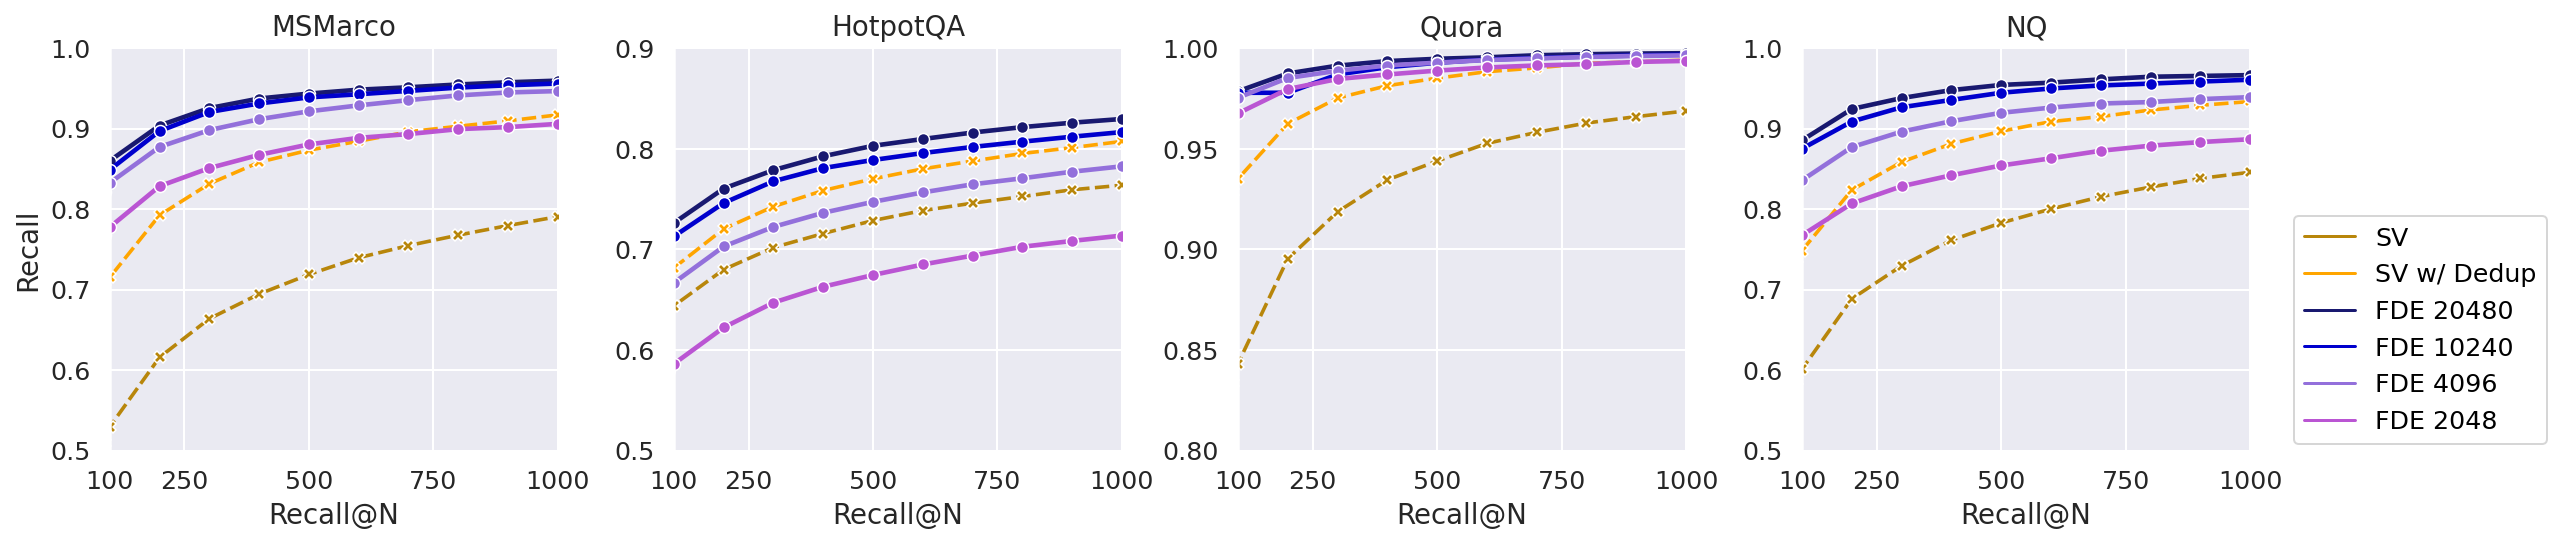
\includegraphics[width=\linewidth]{plots/SV_vs_MV.png}
   \caption{\small FDE retrieval vs SV Heuristic, both with and without document id deduplication. }
         \label{fig:sv_mv} % Add a label (optional)
\end{figure}




\paragraph{Variance.}Note that although the FDE generation is a randomized process, we show in (§\ref{app:variance}) that the variance of the FDE Recall is essentially negligible; for instance, the standard deviation Recall$@$1000 is at most $0.08$-$0.16\%$ for FDEs with $2$-$10k$ dimensions.

